\documentclass{article}
\usepackage{fullpage}
\usepackage{indentfirst}
\usepackage{amsmath}
\usepackage{amsfonts}
\usepackage{rotating}
\usepackage{MnSymbol}
\usepackage{array}
\usepackage{csquotes}
\usepackage{tipa}
\usepackage{tikz}
\usepackage{tikz-qtree}
\usetikzlibrary{matrix, arrows, automata}
\usepackage{gb4e}
\noautomath
\usepackage{verbatim}
%\usepackage[backend=bibtex8]{biblatex}
\usepackage{natbib}
%\addbibresource{references.bib}
\newcommand{\del}{\begin{turn}{55}=\end{turn}}
\newcommand{\Y}{$\checkmark$}
\newcommand{\N}{\ding{55}}
\newcommand{\R}{$\Rightarrow$}
\newcommand\myeq{\mathrel{\stackrel{\makebox[0pt]{\mbox{\normalfont\tiny def}}}{=}}}
\newcommand\se{\small+}
\newcommand{\ap}{\approx}
\newcommand{\all}{\forall}
\title{QP2 Proposal}
\author{Chris Oakden}
\begin{document}
\maketitle
\section{Introduction}
The purpose of this qualifying paper is to address the question: `given two competing grammatical models, how to determine whether they are distinct or notationally-equivalent?' We examine this question specifically by focusing on two models of tonal representation proposed by \citet{Yip1989} and \citet{Bao1990}. These models have been to argued to be distinct representations of tone; there are clear differences in their internal structure, and they are said to make different empirical predictions. \par
Addressing the question of notational-equivalence for these structures, however, is non-trivial for several reasons. No method to date has been established to rigorously compare the \emph{structural} content of competing grammatical models and evaluate them on a theory-internal basis. For example, Bao's model of tonal geometry differs from Yip's in its addition of two nodes to the structure (see \S3); it is not immediately clear whether these differences are substantive or superficial. Often, the task of distinguishing two models of grammar is left to the domain of their empirical predictions, that is, whether or not these theories capture the same set of processes. This, too, can be difficult to evaluate, especially when the full range of processes that is said to distinguish two models' empirical coverage is not well-understood. \par
This qualifying paper analyzes the issue of notational equivalence in a model theoretic framework. Specifically, Yip and Bao representations are defined as relational models, and logical transductions of an explicit complexity threshold are posited over model signatures to translate between them, as well as to formalize attested tonal processes (specifically those which earlier work argues can be represented in one model but not the other). Through a rigorous analysis of the models' structure, we find that the additional nodes in Bao's tonal geometry are \emph{structural analogs} of those already present in Yip's representation. This has ramifications for the formalizability of tonal processes: given this correspondence, there is no process (within a specific complexity threshold) that can be represented in one model but not the other. The main argument of this qualifying paper then is that---contra previous claims---the models are not distinct, but instead are notationally-equivalent. In doing so, we also establish a formally-precise protocol for determining the (non-)equivalence of competing theories of phonological structure in general.\par
There are numerous benefits to this approach. Logical transductions over model signatures provide a means to \emph{translate} between structures and study their structural content. Additionally, fixing the complexity of the logic used to formalize phonological processes allows us to confine model evaluation to a restricted and well-defined space of processes. Empirical predictions made by competing models can thus be compared at a previously unavailable level of explicitness. Perhaps most important is the fact that the logical formalism \emph{unifies} comparison of structure and comparison of empirical coverage by reasoning over them in the same formal language (and with the same complexity; see \S5.2). \par
The remainder of this proposal is as follows. \S2 introduces the notion of notational equivalence, and adopts a definition to be used in analysis. \S3 explores the Yip and Bao tonal geometries, as well as arguments for their categorization as distinct theories of tonal representation. The formal research question and proposal are outlined in \S4, while \S5 details the model theoretic methodology employed in the qualifying paper and its motivations. \S6 lists the remaining steps of the project and proposes a research plan. \S7 concludes.
\section{Notational Equivalence}
There is a tacit assumption in the study of linguistic theory that new theories improve on older ones by increasing both the expressivity and restrictiveness of their predecessors. Models of grammar seek to explain the widest possible scope of attested phenomena, while at the same time limiting their predictive power such that the models do not predict unnatural/impossible/unattested patterns. It follows, then, that new theories do not simply rehash older ones; that is, that the new contribution is distinct from earlier iterations. A reasonable expectation of such contributions is that they predict alternations that are attested in human language, but that earlier theories failed to predict. New contributions to linguistic theory should also mitigate the problems of over-expressivity left by previous theories by reigning in their predictive power. Ideally, they do both simultaneously. \par 
However, if a proposed theory merely restates the generalizations of older theories, or if the former differs from the latter in superficial ways---such that no demonstrable improvement in expressivity/restrictiveness obtains---we may argue that the two are \emph{not} distinct, but rather are notational equivalents of one another. An early discussion of this issue in the literature is due to \citet[p.~2]{Chomsky1972}:
\begin{displayquote}
Given alternative formulations of a theory of grammar, one must first seek to determine how they differ in their empirical consequences, and then try to find ways to compare them in the area of difference. It is easy to be misled into assuming that differently formulated theories actually do differ in empirical consequences, when in fact they are intertranslatable - in a sense, mere notational variants.
\end{displayquote}
A more recent description expands on this definition, identifying three main components by which alternative models can be considered notationally equivalent. One is that they formalize the same set of properties but do not differ significantly in their representation; another is that they share the same empirical coverage; another is a symmetry of equivalence. In other words, a model that is equivalent to another is \citep{Hayes2013}:
\begin{displayquote}
A notational model (for example, a model of a theory of grammar) that represents the same set of abstract properties as an alternative notational model, but in a superficially different way, and which makes the same empirical predictions as the alternative model. (The relation of notational variance is symmetrical - that is, if X is a notational variant of Y, then Y is a notational variant of X.)
\end{displayquote}
In this qualifying paper, we adopt the above definition and apply it to two competing models of tonal representation (those proposed by Yip (1989) and Bao (1989)) which have been claimed to be distinct. The goal here is to determine whether they are indeed different models, or whether they are merely notational equivalents. This is achieved using the formalism of model theory; such an approach quantifies general notions of `superficial difference' and `empirical predictions' in an explicit and formally-rigorous fashion. Further justification for this approach is developed in the following sections, especially \S5.
\section{Tonal Geometry in Yip (1989) and Bao (1990)}
In this section, we introduce the two tonal geometries that serve as the focus of analysis in this qualifying paper. We summarize previous claims that these models are distinct (i.e. \emph{not} notationally equivalent). Specifically, certain types of tonal processes are said to be formalizable using Bao's representation, but not Yip's. The argument goes, then, that the two models do not make the same empirical predictions. We provide an example of such a process, outlining arguments for its representability in Bao's model only. Issues with this generalization are noted, and we motivate an analysis in the model-theoretic formalism to circumvent those issues.
\subsection{Yip (1989)}
Yip (1989) draws on earlier work on the branching structure of affricates to propose a novel model of tonal geometry \citep{Yip1989, Clements1985, Sagey1986}. This model is inspired by characteristics of contour tones which have parallels in the segmental domain, namely association of contour tones as units as well as edge effects. Yip proposes a geometry in which `tonal features hang off a root node', much like Sagey's (1986) branching structure for affricates. The root node associates to a TBU (which Yip argues to be the syllable in Chinese languages) mirroring the association between a consonantal root node and a `C' segment in Sagey's terms. The tonal root itself is a register node specified by the binary feature [$\pm$upper] which bisects the vocal register. This node dominates up to two terminal tonal nodes, specified as [$\pm$raised] (borrowing terminology from \citet{Pulleyblank1986}), further dividing up the vocal space. Contour tones are thus sequences of [+raised][-raised] or [-raised][+raised]. Compare Sagey's model of an affricate to Yip's model of a contour tone below.
\begin{center}
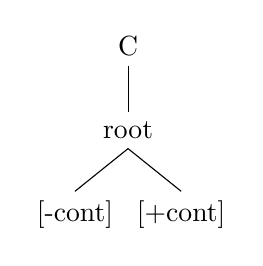
\begin{tikzpicture}[baseline=(current bounding box.north)]
\Tree [.C [.root [.{$[$-cont$]$} ] [.{$[$+cont$]$} ]]];
\end{tikzpicture}
\hspace{1cm}
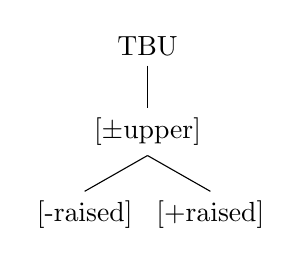
\begin{tikzpicture}[baseline=(current bounding box.north)]
\Tree [.TBU [.{$[\pm$upper$]$} [.{$[$-raised$]$} ] [.{$[$+raised$]$} ]]];
\end{tikzpicture}
\end{center}
Note that the upper bound on root node branching is two; Yip argues that ultra-complex tonal structures (convex [HLH] and concave [LHL]) are the result of multiple root nodes on a single syllable. We restrict the discussion in this qualifying paper to simple contours. \par
Consider an example from Zhenhai, a Wu dialect spoken in Zhenjiang \citep{Chen2000, Rose1990}. The word \textipa{f\~a}$^{11}$\textipa{k\;E}$^{334}$`bedroom' is given the string representation [L.MH]. In Yip's representation, this is a disyllabic form with individual register and terminal tonal nodes.
\begin{center}
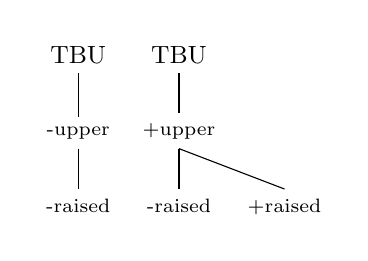
\begin{tikzpicture} [baseline = (z1.base)]
\matrix (m) [matrix of nodes, column sep = .5em, row sep = 1.5em]{
\node(y1){\small TBU}; &   \node(y2){\small TBU}; \\
\node(z1){\scriptsize -upper}; &  \node(z4){\scriptsize +upper}; \\
\node(t1){\scriptsize -raised}; &   \node(t3){\scriptsize -raised}; & \node(t4){\scriptsize +raised}; \\
};
\draw (z1.north) -- (y1.south);
\draw (z1.south) -- (t1.north);
\draw (y2.south) -- (z4.north);
\draw (z4.south) -- (t3.north);
\draw (z4.south) -- (t4.north);
\end{tikzpicture}
\hspace{1cm}
$\equiv$
\hspace{1cm}
[L.MH]
\end{center}
An [L] tone in string representation is a shorthand for a complex of a [-upper] register node dominating a [-raised] terminal node. Similarly, [MH] is a shorthand for a single [+upper] register node which dominates two terminal tonal nodes: [-raised] followed by [+raised].
\subsection{Bao (1990)}
\citet{Bao1990} explores the empirical behavior of tone cross-linguistically and examines the formal relations between tone and other phonological structures to propose a novel tonal geometry. This representation conceptualizes tone as a separate tier on the syllable plane (associating to a TBU via adjunction), but not a separate plane itself. The internal structure of tone differs crucially from Yip's model in two ways. First, the tonal root node and register node (conflated in Yip's tonal geometry) are separate nodes. The root node `T' (`t' in the original, but capitalized here to distinguish it from terminal tonal `t' nodes in our terminology) \emph{dominates} a separate register node which is specified by the laryngeal feature [$\pm$stiff]. This feature is equivalent to Yip's [$\pm$upper] in that it divides the vocal range into two registers. The root node further dominates a `c' or `contour' node which itself dominates up to two terminal tonal nodes, specified [$\pm$slack] in Bao's terms.
\begin{center}
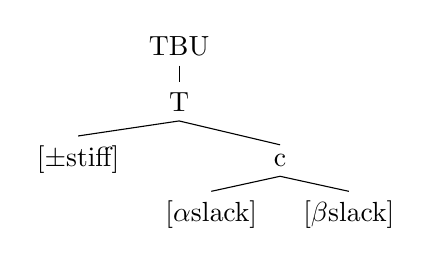
\begin{tikzpicture}[baseline = (current bounding box.north), sibling distance = 10pt]
\tikzset{level distance = 20pt}
\Tree [.TBU [.T [.{$[\pm$stiff$]$} ] [.c [.{$[\alpha$slack$]$} ] [.{$[\beta$slack$]$} ]]]];
\end{tikzpicture}
\end{center}
Much like Yip's [$\pm$raised] feature, sequences of [$\pm$slack] are used to denote rising and falling contours, with single nodes denoting level tones. Bao offers only the formal configuration of `c' terminal nodes above. An implicit upper bound of two on `c' node branching is thus implicit in his model.\par
The same Zhenhai form above can also be represented in Bao's model, that is, the string representation [L.MH] is a multitiered structure comprising `T' root nodes, register and `c' nodes, and terminal nodes:
\begin{center}
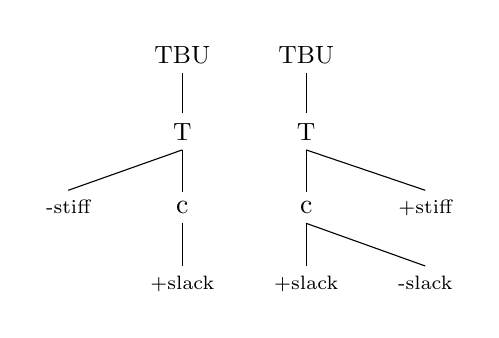
\begin{tikzpicture} [baseline = (y1.base)]
\matrix (m) [matrix of nodes, column sep = 1.5em, row sep = 1.5em]{
& \node(x1){\small TBU}; & \node(x2){\small TBU}; \\
& \node(y1){\small T}; &  \node(y2){\small T}; \\
\node(z1){\scriptsize -stiff}; & \node(z2){c}; & \node(z3){c}; & \node(z4){\scriptsize +stiff}; \\
& \node(t2){\scriptsize +slack}; &  \node(t3){\scriptsize +slack}; & \node(t4){\scriptsize -slack}; \\
};
\draw (x1.south) -- (y1.north);
\draw (x2.south) -- (y2.north);
\draw (z1.north) -- (y1.south);
\draw (z2) -- (y1.south);
\draw (z2.south) -- (t2);
\draw (y2) -- (z3);
\draw (y2.south) -- (z4.north);
\draw (z3) -- (t3);
\draw (z3.south) -- (t4.north);
\end{tikzpicture}
\hspace{1cm}
$\equiv$
\hspace{1cm}
[L.MH]
\end{center}
[L] in string representation is a simplification of a structure headed by a root node `T' dominating a low register [-stiff] node and a `c' node. The `c' node dominates a single [+slack]-featured terminal. Again, as in Yip's representation, [MH] is defined as a single root node whose `c' node dominates two terminal nodes: [+slack] and [-slack].
\subsection{Two Non-Equivalent Models?}
These models of tonal representation are argued to make different typological predictions \citep{Bao1990, Chen2000}. Bao's model in particular is claimed to provide wider empirical coverage, formalizing some processes that cannot be represented in Yip's model. As a result, these models are understood as non-equivalent. \par
\citet[p.~95-6]{Bao1990} motivates a non-root `c' or `contour' node in the representation, identifying the need for a theory which predicts that contours will behave phonologically as units \emph{independent of register}. He substantiates this claim with empirical evidence of contour spread/assimilation, specifically data from Zhenjiang and Wenzhou dialects. Such cases, as Bao argues, can only be accommodated by models for which terminal tonal nodes are not directly dominated by a root node, but rather are sisters under an intermediary node (`c'), thus allowing them to behave as an independent unit.
\begin{center}
(a)
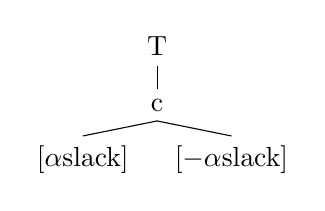
\begin{tikzpicture}[baseline = (current bounding box.north), sibling distance = 10pt]
\tikzset{level distance = 20pt}
\Tree [.T [.c [.{$[\alpha$slack$]$} ] [.{$[-\alpha$slack$]$} ] ]];
\end{tikzpicture}
\hspace{1cm}
(b)
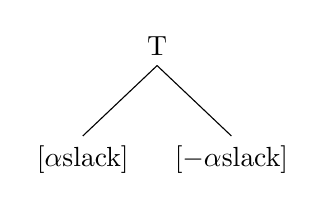
\begin{tikzpicture}[baseline = (current bounding box.north), sibling distance = 10pt]
\tikzset{level distance = 40pt}
\Tree [.T [.{$[\alpha$slack$]$} ] [.{$[-\alpha$slack$]$} ] ];
\end{tikzpicture}
\end{center}
In Yip's model, the tonal root bears register features directly (as in (b) above, where the `t' node would specify either upper or lower register). As such, contour cannot spread without also spreading register information. Yip's model, then, is considered incapable of formalizing patterns exhibiting the independence of contour from register. \par
Chen (2000) echoes this claim with evidence from Zhenhai, a language for which sandhi alternations surface as the shift of contour to an adjacent syllable \citep{Chen2000, Rose1990}. Consider the base and sandhi forms of the Zhenhai word \textipa{f\~a}$^{11}$ \textipa{k\;E}$^{334}$ (the latter of which we have represented above in the respective tonal geometries):
\begin{center}
\begin{tabular}{lllc}
\textipa{f\~a} & \textipa{k\;E} & `bedroom' \\
213 & 441 & base form & /LM.HL/ \\
11 & 334 & sandhi form & [L.MH] \\
\end{tabular}
\end{center}
Per Chen's analysis, the underlying form of this disyllabic structure is /LM.HL/, a low-rising contour followed by a high-falling contour. Sandhi application yields an output form for which the \emph{contour} has shifted one syllable to the right, resulting in a high rising contour [MH]. A default `l' tone is inserted on the leftmost syllable, surfacing as a low-registered low tone [L]. Crucially, both syllables retain their underlying \emph{registers}: [\textipa{f\~a}] is low-registered and [\textipa{k\;E}] is high-registered. \par
Tonal information on an underlying /LM.HL/ structure is definable as follows. The first syllable is a low-rising contour, a [-stiff] register node and a `c' node dominated by a tonal root `T' node. That `c' node dominates a sequence of [+slack] and [-slack] terminals (rising contour). Similarly, in the second syllable (high-falling), a [+stiff] register node and `c' node are sisters under a `T' root, the latter of which dominates a [-slack],[+slack] sequence. Graphically, the model is:
 \begin{center}
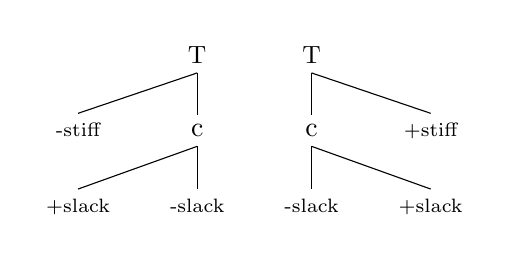
\begin{tikzpicture} [baseline = (y1.base)]
\matrix (m) [matrix of nodes, column sep = 1.5em, row sep = 1.5em]{
& \node(y1){\small T}; &  \node(y2){\small T}; \\
\node(z1){\scriptsize -stiff}; & \node(z2){c}; & \node(z3){c}; & \node(z4){\scriptsize +stiff}; \\
\node(t1){\scriptsize +slack}; & \node(t2){\scriptsize -slack}; &  \node(t3){\scriptsize -slack}; & \node(t4){\scriptsize +slack}; \\
};
\draw (z1.north) -- (y1.south);
\draw (z2) -- (y1.south);
\draw (z2.south) -- (t1.north);
\draw (z2.south) -- (t2);
\draw (y2) -- (z3);
\draw (y2.south) -- (z4.north);
\draw (z3) -- (t3);
\draw (z3.south) -- (t4.north);
\end{tikzpicture}
\end{center}
Contour shift is simply the result of spread and delink. The `c' node on the first syllable spreads to the root of the second syllable, and underlying c-to-T associations delink. 
\begin{center}
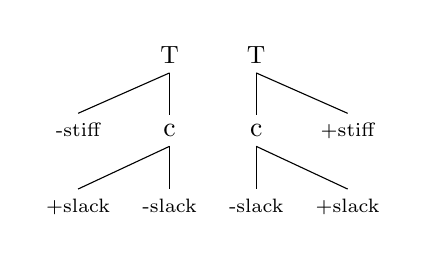
\begin{tikzpicture} [baseline = (z1.base)]
\matrix (m) [matrix of nodes, column sep = .5em, row sep = 1.5em]{
& \node(y1){\small T}; &  \node(y2){\small T}; \\
\node(z1){\scriptsize -stiff}; & \node(z2){c}; & \node(z3){c}; & \node(z4){\scriptsize +stiff}; \\
\node(t1){\scriptsize +slack}; & \node(t2){\scriptsize -slack}; &  \node(t3){\scriptsize -slack}; & \node(t4){\scriptsize +slack}; \\
};
\draw (z1.north) -- (y1.south);
\draw (z2) -- (y1.south);
\draw (z2.south) -- (t1.north);
\draw (z2.south) -- (t2);
\draw (y2) -- (z3);
\draw (y2.south) -- (z4.north);
\draw (z3) -- (t3);
\draw (z3.south) -- (t4.north);
\end{tikzpicture}
\hspace{.3cm}
$\rightarrow$
\hspace{.3cm}
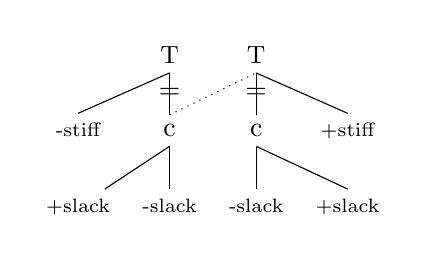
\begin{tikzpicture} [baseline = (z1.base)]
\matrix (m) [matrix of nodes, column sep = .5em, row sep = 1.5em]{
& \node(y1){\small T}; &  \node(y2){\small T}; \\
\node(z1){\scriptsize -stiff}; & \node(z2){c}; & \node(z3){c}; & \node(z4){\scriptsize +stiff}; \\
\node(t1){\scriptsize +slack}; & \node(t2){\scriptsize -slack}; &  \node(t3){\scriptsize -slack}; & \node(t4){\scriptsize +slack}; \\
};
\draw (z1.north) -- (y1.south);
\path (z2) edge node{=} (y1);
\draw (z2.south) -- (t1);
\draw (z2) -- (t2);
\path (z3) edge node{=} (y2);
\draw (y2.south) -- (z4.north);
\draw (z3) -- (t3.north);
\draw (z3.south) -- (t4.north);
\draw [dotted] (z2.north) -- (y2.south);
\end{tikzpicture}
\end{center}
Finally, a default `l' ([+slack]) attaches to the first syllable.\footnote{This should be a complex of a `c' node and a terminal node, since the original first-syllable `c' node is associated to the root node on the final syllable. This detail is not directly relevant now, and we will address it in subsequent sections.} These processes derive the predicted output form [L.MH]. Note that the register nodes are undisturbed by contour spread; underlying register feature designations are preserved in the output.
\begin{center}
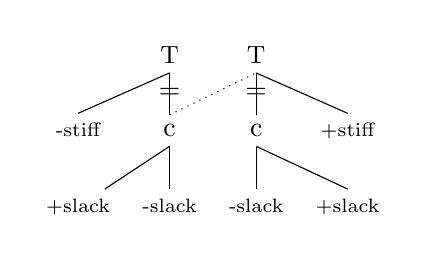
\begin{tikzpicture} [baseline = (z1.base)]
\matrix (m) [matrix of nodes, column sep = .5em, row sep = 1.5em]{
& \node(y1){\small T}; &  \node(y2){\small T}; \\
\node(z1){\scriptsize -stiff}; & \node(z2){c}; & \node(z3){c}; & \node(z4){\scriptsize +stiff}; \\
\node(t1){\scriptsize +slack}; & \node(t2){\scriptsize -slack}; &  \node(t3){\scriptsize -slack}; & \node(t4){\scriptsize +slack}; \\
};
\draw (z1.north) -- (y1.south);
\path (z2) edge node{=} (y1);
\draw (z2.south) -- (t1);
\draw (z2) -- (t2);
\path (z3) edge node{=} (y2);
\draw (y2.south) -- (z4.north);
\draw (z3) -- (t3.north);
\draw (z3.south) -- (t4.north);
\draw [dotted] (z2.north) -- (y2.south);
\end{tikzpicture}
\hspace{.3cm}
$\rightarrow$
\hspace{.3cm}
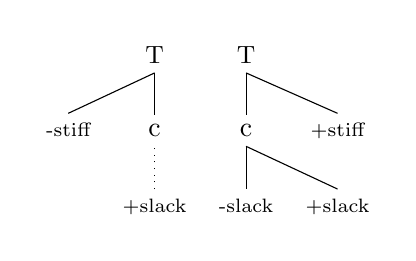
\begin{tikzpicture} [baseline = (z1.base)]
\matrix (m) [matrix of nodes, column sep = .5em, row sep = 1.5em]{
& \node(y1){\small T}; &  \node(y2){\small T}; \\
\node(z1){\scriptsize -stiff}; & \node(z2){c}; & \node(z3){c}; & \node(z4){\scriptsize +stiff}; \\
&\node(t1){\scriptsize +slack};  &  \node(t3){\scriptsize -slack}; & \node(t4){\scriptsize +slack}; \\
};
\draw (z1.north) -- (y1.south);
\draw (z2) -- (y1);
\draw (y2) -- (z3);
\draw (y2.south) -- (z4.north);
\draw (z3) -- (t3);
\draw (z3.south) -- (t4.north);
\draw [dotted] (t1) -- (z2);
\end{tikzpicture}
\end{center} \par
The Zhenhai case is argued to provide direct evidence of the non-equivalency of the two models. Performing the same spread and delink procedure on Yip's tonal geometry would ostensibly entail carriage of register information along with contour information, an undesired result. This is due to the fact that the immediate dominator of terminal tonal nodes in Yip's model is precisely the node which carries register information. Additionally, this node is also the tonal root node which associates to the TBU; there is no procedural difference, then, between register spread, contour spread, or whole tone spread. The only available option (at a higher level than individual terminal nodes) is spread of a register (root) node to an adjacent TBU. In terms of the Zhenhai contour shift example above, then:
\begin{center}
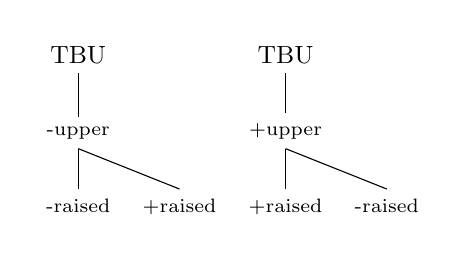
\begin{tikzpicture} [baseline = (z1.base)]
\matrix (m) [matrix of nodes, column sep = .5em, row sep = 1.5em]{
\node(y1){\small TBU}; & &  \node(y2){\small TBU}; \\
\node(z1){\scriptsize -upper}; & & \node(z4){\scriptsize +upper}; \\
\node(t1){\scriptsize -raised}; & \node(t2){\scriptsize +raised}; &  \node(t3){\scriptsize +raised}; & \node(t4){\scriptsize -raised}; \\
};
\draw (z1.north) -- (y1.south);
\draw (z1.south) -- (t1.north);
\draw (z1.south) -- (t2.north);
\draw (y2.south) -- (z4.north);
\draw (z4.south) -- (t3.north);
\draw (z4.south) -- (t4.north);
\end{tikzpicture}
\hspace{.3cm}
$\rightarrow$
\hspace{.3cm}
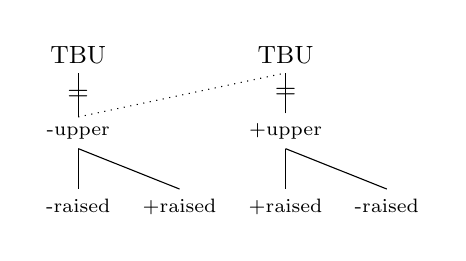
\begin{tikzpicture} [baseline = (z1.base)]
\matrix (m) [matrix of nodes, column sep = .5em, row sep = 1.5em]{
\node(y1){\small TBU}; & &  \node(y2){\small TBU}; \\
\node(z1){\scriptsize -upper}; & & \node(z4){\scriptsize +upper}; \\
\node(t1){\scriptsize -raised}; & \node(t2){\scriptsize +raised}; &  \node(t3){\scriptsize +raised}; & \node(t4){\scriptsize -raised}; \\
};
\path (z1.north) edge node{=} (y1.south);
\path (z4.north) edge node{=} (y2.south);
\draw [dotted] (z1.north) -- (y2.south);
\draw (z1.south) -- (t1.north);
\draw (z1.south) -- (t2.north);
\draw (z4.south) -- (t3.north);
\draw (z4.south) -- (t4.north);
\end{tikzpicture}
\end{center}
The predicted output for this structure (after default `l' insertion) is *[L.LH], as low register spreads with rising contour onto the second syllable. Chen concludes that the Yip and Bao tonal geometries do not make the same empirical predictions (that is, they cannot model the same attested classes of process). Implicit in this claim is the assertion that they are non-equivalent.\par
A theoretically-possible alternative analysis has contour spreading from the terminal tier only. This entails two iterations of tonal node spread, one for each node which together creates a contour. Is this tenable? Neither Chen nor Bao entertain such an analysis, but there is reason to believe that it does not work, either. Specifically, with respect to conventional views on spread and delink processes (e.g. Odden 2001), simultaneous spreading of terminal nodes would be a violation of the No-Crossing Constraint or NCC \citep{Odden2001, Goldsmith1976}.
\begin{center}
\begin{tabular}{cccc}
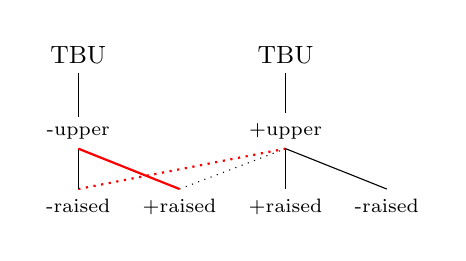
\begin{tikzpicture} [baseline = (z1.base)]
\matrix (m) [matrix of nodes, column sep = .5em, row sep = 1.5em]{
\node(y1){\small TBU}; & &  \node(y2){\small TBU}; \\
\node(z1){\scriptsize -upper}; & & \node(z4){\scriptsize +upper}; \\
\node(t1){\scriptsize -raised}; & \node(t2){\scriptsize +raised}; &  \node(t3){\scriptsize +raised}; & \node(t4){\scriptsize -raised}; \\
};
\draw (z1.north) -- (y1.south);
\draw (z4.north) -- (y2.south);
\draw [color = red, thick, dotted] (t1.north) -- (z4.south);
\draw [dotted] (t2.north) -- (z4.south);
\draw (z1.south) -- (t1.north);
\draw [thick, color = red](z1.south) -- (t2.north);
\draw (z4.south) -- (t3.north);
\draw (z4.south) -- (t4.north);
\end{tikzpicture}
&
$\rightarrow$
&
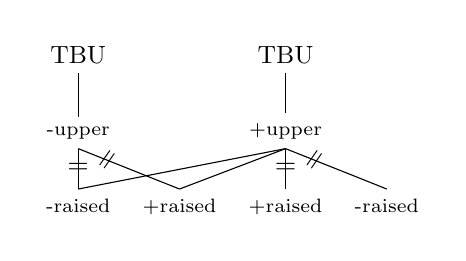
\begin{tikzpicture} [baseline = (z1.base)]
\matrix (m) [matrix of nodes, column sep = .5em, row sep = 1.5em]{
\node(y1){\small TBU}; & &  \node(y2){\small TBU}; \\
\node(z1){\scriptsize -upper}; & & \node(z4){\scriptsize +upper}; \\
\node(t1){\scriptsize -raised}; & \node(t2){\scriptsize +raised}; &  \node(t3){\scriptsize +raised}; & \node(t4){\scriptsize -raised}; \\
};
\draw (z1.north) -- (y1.south);
\draw (z4.north) -- (y2.south);
\draw (t1.north) -- (z4.south);
\draw (t2.north) -- (z4.south);
\path (z1.south) edge node{=} (t1.north);
\path (z1.south) edge node[pos=.3]{\del} (t2.north);
\path (z4.south) edge node{=} (t3.north);
\path (z4.south) edge node[pos=.3]{\del} (t4.north);
\end{tikzpicture}
&
(Spread + Delink) \\
&
&
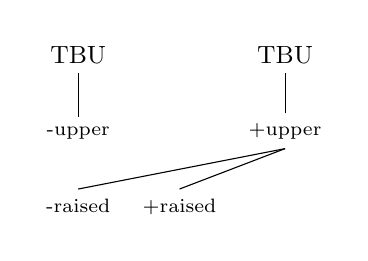
\begin{tikzpicture} [baseline = (z1.base)]
\matrix (m) [matrix of nodes, column sep = .5em, row sep = 1.5em]{
\node(y1){\small TBU}; & &  \node(y2){\small TBU}; \\
\node(z1){\scriptsize -upper}; & & \node(z4){\scriptsize +upper}; \\
\node(t1){\scriptsize -raised}; & \node(t2){\scriptsize +raised}; \\
};
\draw (z1.north) -- (y1.south);
\draw (z4.north) -- (y2.south);
\draw (t1.north) -- (z4.south);
\draw (t2.north) -- (z4.south);
\end{tikzpicture}
&
(Output) \\
\end{tabular}
\end{center}
On the assumption that, in a derivation, spread occurs \emph{before} delink, contour shift as terminal node spread violates the NCC; the leftmost terminal tonal node in the first syllable (dotted red) crosses the tautosyllabic terminal node association (solid red) while spreading. \par
But what about a piece-meal process in which one terminal spreads and delinks, then another spreads and delinks? In other words, the process is two iterations of \emph{spread and delink}.
\begin{center}
\begin{tabular}{cccc}
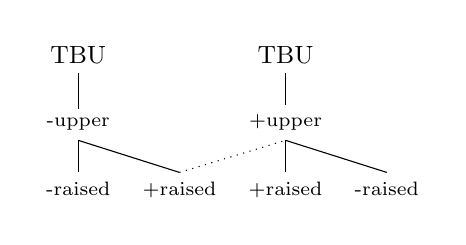
\begin{tikzpicture} [baseline = (z1.base)]
\matrix (m) [matrix of nodes, column sep = .5em, row sep = 1.2em]{
\node(y1){\small TBU}; & &  \node(y2){\small TBU}; \\
\node(z1){\scriptsize -upper}; & & \node(z4){\scriptsize +upper}; \\
\node(t1){\scriptsize -raised}; & \node(t2){\scriptsize +raised}; &  \node(t3){\scriptsize +raised}; & \node(t4){\scriptsize -raised}; \\
};
\draw (z1.north) -- (y1.south);
\draw (z4.north) -- (y2.south);
\draw [dotted] (t2.north) -- (z4.south);
\draw (z1.south) -- (t1.north);
\draw (z1.south) -- (t2.north);
\draw (z4.south) -- (t3.north);
\draw (z4.south) -- (t4.north);
\end{tikzpicture}
&
$\rightarrow$
&
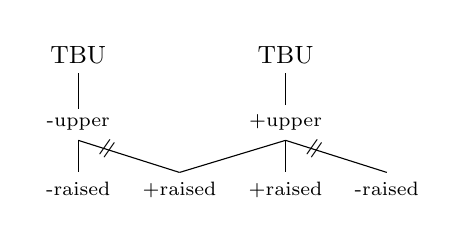
\begin{tikzpicture} [baseline = (z1.base)]
\matrix (m) [matrix of nodes, column sep = .5em, row sep = 1.2em]{
\node(y1){\small TBU}; & &  \node(y2){\small TBU}; \\
\node(z1){\scriptsize -upper}; & & \node(z4){\scriptsize +upper}; \\
\node(t1){\scriptsize -raised}; & \node(t2){\scriptsize +raised}; &  \node(t3){\scriptsize +raised}; & \node(t4){\scriptsize -raised}; \\
};
\draw (z1.north) -- (y1.south);
\draw (z4.north) -- (y2.south);
\draw (t2.north) -- (z4.south);
\draw (z1.south) -- (t1.north);
\path (z1.south) edge node[pos=.3]{\del} (t2.north);
\draw (z4.south) -- (t3.north);
\path (z4.south) edge node[pos=.3]{\del} (t4.north);
\end{tikzpicture}
&
(Spread + Delink 1) \\
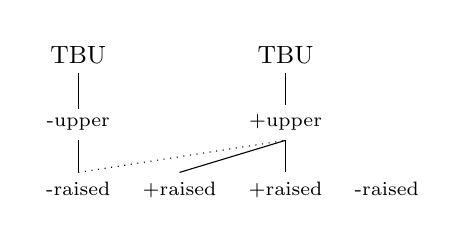
\begin{tikzpicture} [baseline = (z1.base)]
\matrix (m) [matrix of nodes, column sep = .5em, row sep = 1.2em]{
\node(y1){\small TBU}; & &  \node(y2){\small TBU}; \\
\node(z1){\scriptsize -upper}; & & \node(z4){\scriptsize +upper}; \\
\node(t1){\scriptsize -raised}; & \node(t2){\scriptsize +raised}; &  \node(t3){\scriptsize +raised}; & \node(t4){\scriptsize -raised}; \\
};
\draw (z1.north) -- (y1.south);
\draw (z4.north) -- (y2.south);
\draw [dotted] (t1.north) -- (z4.south);
\draw (t2.north) -- (z4.south);
\draw (z1.south) -- (t1.north);
\draw (z4.south) -- (t3.north);
\end{tikzpicture}
&
$\rightarrow$
&
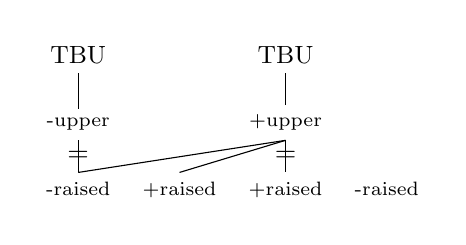
\begin{tikzpicture} [baseline = (z1.base)]
\matrix (m) [matrix of nodes, column sep = .5em, row sep = 1.2em]{
\node(y1){\small TBU}; & &  \node(y2){\small TBU}; \\
\node(z1){\scriptsize -upper}; & & \node(z4){\scriptsize +upper}; \\
\node(t1){\scriptsize -raised}; & \node(t2){\scriptsize +raised}; &  \node(t3){\scriptsize +raised}; & \node(t4){\scriptsize -raised}; \\
};
\draw (z1.north) -- (y1.south);
\draw (z4.north) -- (y2.south);
\draw (t1.north) -- (z4.south);
\draw (t2.north) -- (z4.south);
\path (z1.south) edge node{=} (t1.north);
\path (z4.south) edge node{=} (t3.north);
\end{tikzpicture}
&
(Spread + Delink 2) \\
&
&
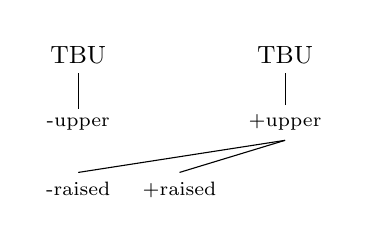
\begin{tikzpicture} [baseline = (z1.base)]
\matrix (m) [matrix of nodes, column sep = .5em, row sep = 1.2em]{
\node(y1){\small TBU}; & &  \node(y2){\small TBU}; \\
\node(z1){\scriptsize -upper}; & & \node(z4){\scriptsize +upper}; \\
\node(t1){\scriptsize -raised}; & \node(t2){\scriptsize +raised}; \\
};
\draw (z1.north) -- (y1.south);
\draw (z4.north) -- (y2.south);
\draw (t1.north) -- (z4.south);
\draw (t2.north) -- (z4.south);
\end{tikzpicture}
&
(Output) \\
\end{tabular}
\end{center}
This instantiation of spread and delink would not violate the NCC. There are, however, problems with this approach. First, we lose the intuition here that contour is spreading \emph{as a unit}; spread and delink is divided into separate (and crucially-ordered) processes (recall that Bao's representation is perfectly well-formed without it). In addition, we cannot be sure that the piece-meal process is even predicted by theories of spread and delink, or whether it is of the same computational complexity as the simultaneous analog. An analysis like the one above subdivides the already ill-defined question of possible vs impossible processes into two additional possibilities. On one hand is the question of whether it is possible at all to model a certain process; on the other is the question of whether a possible representation is somehow unattractive from a theoretical point of view, or misses the mark on the intuition the generalization hopes to capture. This only serves to further obscure the question itself. To date, there is no comprehensive typological work surveying the full range of spread and delink processes that would shed light on these issues, and such an undertaking is not within the scope of this qualifying paper. It is worth noting, though, that a key argument for the non-equivalence of the two models centers on a process which has not been fully explored in the literature. \par
The advantage of analyzing these processes in the formalism of model theory and logical transductions, then, is that it allows us to explicitly quantify the question of what processes are `possible' or `impossible' to represent in a particular model (i.e. their `empirical coverage'). As the full range of spread and delink processes is not fully understood, we can only reason over the processes as they are presented in previous analyses. By imposing a threshold on the \emph{logical complexity} of their representation, though, it is possible to directly compare the two representations---narrowing on a well-defined subset of the space of processes they model---and answer the question of their equivalence in a principled way. That is the main focus of this qualifying paper. 
\section{Research Question/Proposal}
This QP will address the following research question: are the Yip and Bao tonal geometries notationally equivalent? Previous work has suggested that they are distinct, but the models have yet to be compared in a formally/mathematically rigorous fashion. With the definition of notational equivalence in \S 2 in mind, we will show that these models are demonstrably equivalent. Two main arguments support this claim.\par
First, we will prove that the Yip and Bao geometries are intertranslatable; crucially, one model can be translated into the other \emph{and vice versa}. Both models share the same set of basic properties, but differ in terms of how those properties are structured. These differences in structure are superficial, however; translating between the representations is straightforward and can be achieved using simple logic (see \S5). We offer translations between models which capitalize on a number of structural and featural equivalencies between them. Specifically, we portray Yip's register node ($\pm$upper) as a \emph{fusion} of Bao's root `T', register, and `c' nodes. This register node is the structural analog of Bao's `T' root node (associates with a TBU) and `c' node (dominates terminal tonal nodes), and the featural equivalent of Bao's register node ($\pm$stiff) in that it bisects the pitch range. TBU and terminal nodes are also argued to be both structurally and featurally analogous across models. This is shown below where `SE' indicates structural equivalence, `FE' indicates featural equivalence, and `SE/FE' indicates both.
\begin{center}
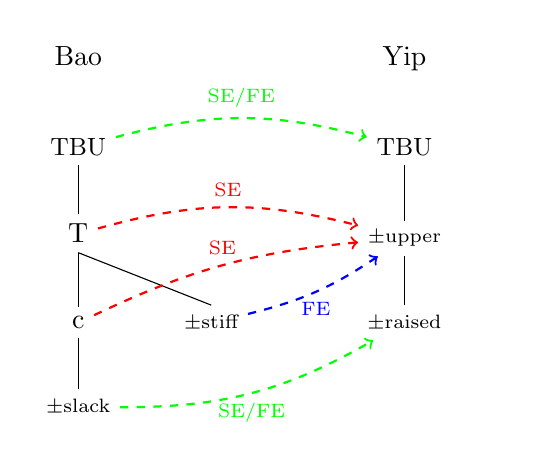
\begin{tikzpicture} [baseline = (x.base)]
\matrix (m) [matrix of nodes, column sep = 2em, row sep = 1.8em]{
Bao & & & Yip \\
\node(x){\small TBU}; & & &  \node(x2){\small TBU};\\
\node(y){T}; & & & \node(y2){\scriptsize $\pm$upper};& \\
\node(z){c}; & \node(z2){\scriptsize $\pm$stiff};& & \node(z3){\scriptsize $\pm$raised};& \\
\node(t){\scriptsize $\pm$slack};& \\
};
\draw (x) -- (y);
\draw (x2) -- (y2);
\draw (z) -- (y) ;
\draw (z2.north) -- (y.south) ;
\draw (z3) -- (y2) ;
\draw (t) -- (z) ;
\path [color = green, thick, dashed, ->] (x) edge[bend left=15] node[above]{\scriptsize SE/FE} (x2);
\path [color = red, thick, dashed, ->] (y) edge[bend left=15] node[above]{\scriptsize SE} (y2);
\path [color = blue, thick, dashed, ->] (z2) edge[bend right=10] node[below]{\scriptsize FE} (y2);
\path [color = red, thick, dashed, ->] (z) edge[bend left=10] node[above]{\scriptsize SE} (y2);
\path [color = green, thick, dashed, ->] (t) edge[bend right=15] node[below]{\scriptsize SE/FE} (z3);
\end{tikzpicture}
\end{center}
A translation from Yip's representation to Bao's, then, is the inverse, that is, an \emph{explosion} of a single register node into a complex of three nodes which contain the structural and featural information of that node. The first node in this complex is the `T' node encoding the structural position of the node to which a TBU associates (i.e. tonal root). The `c' node represents the position of immediate dominator of tonal terminals. Register \emph{features} on this node ($\pm$upper) are contained in a separate node ($\pm$stiff) which contains neither of the structural properties mentioned above. 
\begin{center}
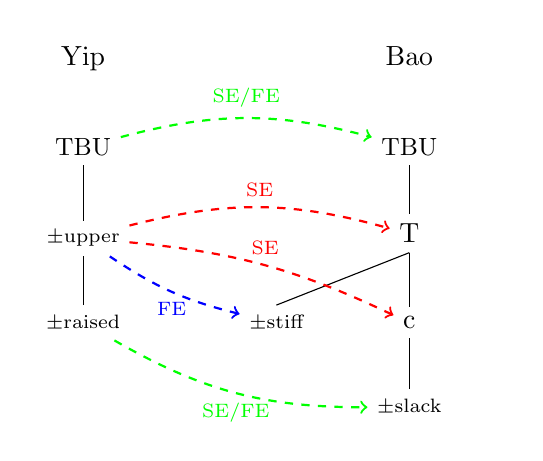
\begin{tikzpicture} [baseline = (x.base)]
\matrix (m) [matrix of nodes, column sep = 2em, row sep = 1.8em]{
Yip & & & Bao \\
\node(x){\small TBU}; & & &  \node(x2){\small TBU};\\
\node(y){\scriptsize $\pm$upper}; & & & \node(y2){T};& \\
\node(z){\scriptsize $\pm$raised}; & & \node(z2){\scriptsize $\pm$stiff};& \node(z3){c};& \\
& & & \node(t){\scriptsize $\pm$slack};& \\
};
\draw (x) -- (y);
\draw (x2) -- (y2);
\draw (z) -- (y) ;
\draw (z2.north) -- (y2.south) ;
\draw (z3) -- (y2) ;
\draw (t) -- (z3) ;
\path [color = green, thick, dashed, ->] (x) edge[bend left=15] node[above]{\scriptsize SE/FE} (x2);
\path [color = red, thick, dashed, ->] (y) edge[bend left=15] node[above]{\scriptsize SE} (y2);
\path [color = blue, thick, dashed, ->] (y) edge[bend right=10] node[below]{\scriptsize FE} (z2);
\path [color = red, thick, dashed, ->] (y) edge[bend left=10] node[above]{\scriptsize SE} (z3);
\path [color = green, thick, dashed, ->] (z) edge[bend right=15] node[below]{\scriptsize SE/FE} (t);
\end{tikzpicture}
\end{center}
Translations between models will be performed as graph transductions (see \S 5); we will show that these are straightforward and achievable with a low threshold of logical complexity, supporting the claim that Yip and Bao representations are notationally equivalent.\par
Additionally, we will argue that---as a result of this intertranslatability, and contra previous studies---these models make the same empirical predictions. That is to say, given that the differences between Bao and Yip representations are trivial, there are no tonal processes formalizable in one model but not the other. As a starting point, we focus on tone sandhi processes in Chinese dialects, with the understanding that future work will extend the typological scope of processes and tonal systems. Crucially, we examine the spread/shift patterns that are argued to be predicted by Bao's model but not Yip's, for example, spread/shift of contour that is independent of register, including tone sandhi alternations in Zhenhai, Zhenjiang, and Wenzhou \citep{Bao1990, Chen2000}. Other common tone sandhi processes include spread/shift patterns that target register, whole contour tones, and terminal nodes; dissimilation and substitution; and neutralization. \par
Analysis of these processes and how they can be formalized in both models is made explicit through the use of logical transductions between input and output structures in both models. Sandhi patterns are therefore formalized as functions which take a tonal geometric base form input and output a corresponding sandhi form (see \S 5).
\section{Methodology}
This section introduces the methodological framework the qualifying paper will adopt to prove the notational equivalence of Yip and Bao tonal representations. Tonal geometries are first represented as relational models using model theory; the individual components of each tonal geometry and their internal structure are thus given a precise representation. With these definitions in hand, we can then address the question of their equivalence, that is, their intertranslatability and the extent to which they make the same empirical predictions. This is achieved via logical transductions. Logical transductions give us the ability to translate between the representations and identify their structural/featural analogs (see \S4). Additionally, they offer a means to model tonal processes as input-output maps in a formally-rigorous fashion. By limiting the expression of these processes to a specific threshold of logical complexity, we compare the models over a restricted range of possible/impossible processes, thereby mitigating the issues raised in \S3.3. \par
We prove that both varieties of transduction are definable using Quantifier-Free (QF) First Order logic, a simple and restrictive logic. In doing so, we quantify notions of `superficial' differences between representations and `process formalizability' in explicit mathematical terms (logical complexity), as well as provide a way to discuss two separate components of notational equivalence--intertranslatability and empirical predictions--using the same formal language.
\subsection{Model Theory}
Tonal geometries, in general terms, can be described as structures with related elements. Elements carry a specific feature in the representation (TBUs, root nodes, register/contour nodes, terminal tonal nodes), and certain elements relate to one another (TBUs and tonal roots associate, root nodes dominate register nodes or tonal nodes, syllables are in a linear order, etc.). In this qualifying paper, we use model theory to represent these structures. This allows for an explicit description of the representations as mathematical objects.\par
Specifically, we represent tonal geometries in terms of relational models. A relational model comprises a domain of elements and a set of their relations defined over some universe of elements (e.g., an alphabet $\Sigma$). For example, we can represent the word `pop' as a relational string model defined over an alphabet $\Sigma$ = \{o,p\}. Let such a model $\mathcal{M}_{pop}$ be defined as $\mathcal{M}_{pop}\myeq \langle \mathcal{D}; P_{o}, P_{p};succ(x) \rangle$. The domain $\mathcal{D}$ contains a set of numbers denoting individual elements in the model (string positions in this case); linear order is imposed on the elements via a unary successor function (succ(x)/$\vartriangleleft$) which identifies the position immediately following a given domain element (the final element is its own successor); $P_{o}$ and $P_{p}$ are instantiations of $(P_{\sigma})_{\sigma\in\Sigma}$, unary relations which label elements with a particular feature (in this case the property of being a `p' or an `o'). The model is thus:
\begin{equation}
\begin{aligned}
&\mathcal{M}_{pop} \\
\mathcal{D} &= \{1,2,3\} & P_{o}&= \{2\} & P_{p}&=\{1,3\} & succ(x) &= \begin{cases} 2 & x=1 \\ 3 & x\in\{2,3\} \end{cases}  \\  
\end{aligned}
\end{equation}
Graphically, the model is:
\begin{center}
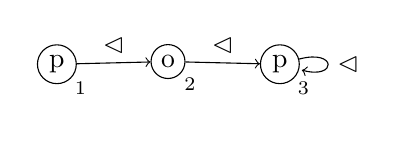
\begin{tikzpicture}[baseline = (x1.base)]
\matrix (m) [matrix of nodes, column sep = 2em]{
\node[draw, circle, inner sep = 2, label = {[label distance = -3pt] below right:\scriptsize 1}](x1){p}; & \node[draw, circle, inner sep = 2, label = {[label distance = -3pt] below right:\scriptsize 2}](x2){o}; & \node[draw, circle, inner sep = 2, label = {[label distance = -3pt] below right:\scriptsize 3}](x3){p}; \\
};
\draw [->] (x1) -- (x2) node[above, pos=.5]{$\vartriangleleft$};
\draw [->] (x2) -- (x3) node[above, pos=.5]{$\vartriangleleft$};
\path [->] (x3) edge[loop right] node{$\vartriangleleft$} (x3);
\end{tikzpicture}
\end{center}
Relational models define the properties of Bao and Yip tonal geometries in an explicit and precise way. These models are defined over alphabets containing all the component featural labels of each representation. As above, unary relations label model elements: TBUs, tonal root nodes, register nodes, etc. Internal structural relations between model elements are described via a set of functions. These include functions for TBU-tonal root association, as well as dominance between root node and register/`c' nodes (in Bao's model), register node and terminal nodes (in Yip's model), and `c' nodes and terminal tonal nodes (in Bao's model). \par
With these functions, then, we can represent not only a single string of symbols, but also several tiers of strings which interrelate (i.e. a multitiered tonal model). A Yip representational model, for example, is a structure with three tiers of strings (TBU, register, tonal terminal) related via functions ($\alpha(x)$ for association, $\delta(x)$ for dominance). We can define a low tone ([-upper] register, [-raised] tone) as a model $\mathcal{M}^{Y}_{l}$ over the alphabet $\Sigma = \{TBU, +upper, -upper, +raised, -raised\}$ as:\footnote{We abstract away from linear order in this example, but analysis of models in this QP will impose an order on elements of the same tier, that is, TBUs, register nodes, terminal tonal nodes, etc.} 
\begin{equation}
\begin{aligned}
&\mathcal{M}^{Y}_{l} \\
\mathcal{D}&= \{1,2,3\} & P_{TBU}&=\{1\} & P_{+upper}&=\{\,\} \\
P_{-upper}&=\{2\} & P_{-raised}&=\{3\} & P_{+raised}&=\{\,\} \\
\alpha(x)&= \begin{cases} 2 & x=1\end{cases} & \delta(x)&= \begin{cases} 2 & x=3 \end{cases}\\
\end{aligned}
\end{equation}
This model mirrors the same tone in Yip's representation.
\begin{center}
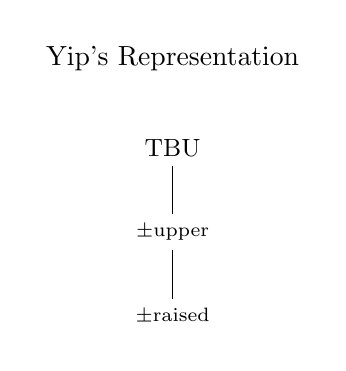
\begin{tikzpicture} [baseline = (x.base)]
\matrix (m) [matrix of nodes, column sep = 2em, row sep = 1.8em]{
Yip's Representation \\
\node(x){\small TBU}; \\
\node(y){\scriptsize $\pm$upper}; \\
\node(z){\scriptsize $\pm$raised}; \\
};
\draw (x) -- (y);
\draw (z) -- (y);
\end{tikzpicture}
\hspace{2cm}
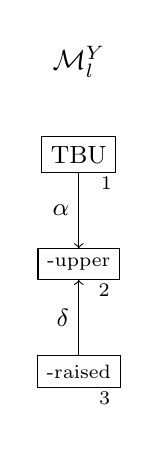
\begin{tikzpicture} [baseline = (x.base)]
\matrix (m) [matrix of nodes, column sep = 2em, row sep = 1.8em]{
$\mathcal{M}^{Y}_{l}$ \\
\node[draw, rectangle,label = {[label distance = -3pt] below right:\scriptsize 1}](x){\small TBU}; \\
\node[draw, rectangle,label = {[label distance = -3pt] below right:\scriptsize 2}](y){\scriptsize -upper}; \\
\node[draw, rectangle,label = {[label distance = -3pt] below right:\scriptsize 3}](z){\scriptsize -raised}; \\
};
\draw [->](x) -- (y) node[left, pos=.5]{\small$\alpha$};
\draw [->](z) -- (y) node[left, pos=.5]{\small$\delta$};
\end{tikzpicture}
\end{center}
Conceptualizing Bao and Yip tonal geometries explicitly allows us to examine the basic structural properties of each. With these models, we can attempt to \emph{translate} between the models. We perform this procedure using logical transductions, described in the next subsection.
\subsection{Logical Transductions and Complexity}
We prove the equivalence of the Bao and Yip representations in part by demonstrating their intertranslatability. In other words, we show that they contain the same set of abstract properties, and differ only in superficial ways. To do so, we define logical transductions that allow us to translate between model theoretic representations of each tonal geometry. \par
These transductions are a mapping from an input signature (of one model) to an output signature (of another model). They are defined via a set of logical formulas. A separate formula is defined for each relation/function in the output signature, and the formulas are interpreted with respect to the logical language of the input signature \citep{Courcelle1994, EngHoo2001}. \par
Logical transductions can also be used to represent a variety of phonological processes as input-to-output maps. We illustrate with an example. Suppose we want to model final devoicing on the word `bob' such that /bob/ $\mapsto$ [bop]. Let this mapping be a logical transduction $\tau$ from the signature $\zeta_{bob}$ of the model $\mathcal{M}_{bob}$ to the signature $\zeta_{bop}$ of the model $\mathcal{M}_{bop}$. In the set of predicates below, `prime' ($'$) indicates output relations. We also add an auxiliary relation based on the definition of successor:
\begin{equation}
\begin{aligned}
last(x) &\myeq succ(x)=x\\
\zeta_{bob}&\myeq \{P_{b}, P_{o},succ\} \\
\zeta_{bop}&\myeq \{P'_{b}, P'_{p}, P'_{o},succ'\} \\
\tau&\myeq \zeta_{bob} \mapsto \zeta_{bop} \\
\end{aligned}
\end{equation}
\begin{equation}
\begin{aligned}
P'_{b}(x)&\myeq P_{b}(x) \land \neg last(x) \\
P'_{p}(x)&\myeq P_{b}(x) \land last(x)\\
P'_{o}(x)&\myeq P_{o}(x) \\
succ'(x) &\myeq succ(x) \\
\end{aligned}
\end{equation}
Applying this transduction to the input model will replace a final `b' with a `p', leaving other elements and relations unchanged (e.g. no change in linear order, `o's or non-final `b's).
\begin{center}
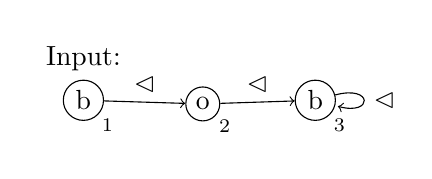
\begin{tikzpicture}[baseline = (x1.base)]
\matrix (m) [matrix of nodes, column sep = 2em]{
Input: \\
\node[draw, circle, inner sep = 2, label = {[label distance = -3pt] below right:\scriptsize 1}](x1){b}; & \node[draw, circle, inner sep = 2, label = {[label distance = -3pt] below right:\scriptsize 2}](x2){o}; & \node[draw, circle, inner sep = 2, label = {[label distance = -3pt] below right:\scriptsize 3}](x3){b}; \\
};
\draw [->] (x1) -- (x2) node[above, pos=.5]{$\vartriangleleft$};
\draw [->] (x2) -- (x3) node[above, pos=.5]{$\vartriangleleft$};
\path [->] (x3) edge[loop right] node{$\vartriangleleft$} (x3);
\end{tikzpicture}
\hspace{.5cm}
$\mapsto$
\hspace{.5cm}
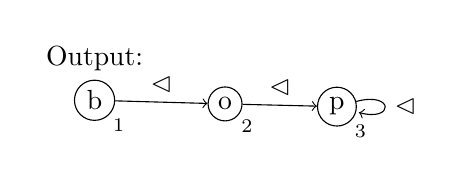
\begin{tikzpicture}[baseline = (x1.base)]
\matrix (m) [matrix of nodes, column sep = 2em]{
Output: \\
\node[draw, circle, inner sep = 2, label = {[label distance = -3pt] below right:\scriptsize 1}](x1){b}; & \node[draw, circle, inner sep = 2, label = {[label distance = -3pt] below right:\scriptsize 2}](x2){o}; & \node[draw, circle, inner sep = 2, label = {[label distance = -3pt] below right:\scriptsize 3}](x3){p}; \\
};
\draw [->] (x1) -- (x2) node[above, pos=.5]{$\vartriangleleft$};
\draw [->] (x2) -- (x3) node[above, pos=.5]{$\vartriangleleft$};
\path [->] (x3) edge[loop right] node{$\vartriangleleft$} (x3);
\end{tikzpicture}
\end{center}
Note here that there is not a complete overlap between the unary predicates in the output and their interpretation in terms of the input structure; the output contains the unary relation $P'_{p}$ which would label an element not present in the input. We will encounter this in the transduction from Yip's model to Bao's model. Relations which label units such as the terminal `T' and contour `c' nodes are not represented explicitly in Yip's model, but there are \emph{structural analogs} of those nodes in Yip's representation (i.e. the `register node'). To define multiple output nodes in terms of a single input node (recall the `explosion' in the previous section), we define the transduction over \emph{multiple copies} of the input. The structural position of Bao's `T' node is defined from a register node in one Yip copy, the structural position of Bao's `c' node is defined from a register node in another Yip copy, and so on. \par
This qualifying paper proves the equivalence of Yip and Bao tonal geometries---thereby establishing a precise method for proving notational equivalence in general---with the use of logical transductions. It does so in two distinct ways. First, we define logical transductions to translate between models and identify their structural and featural analogs (discussed below). We also use logical transductions to model tonal processes as input-output maps (see \S5.3), and evaluate the extent to which respective models can formalize those processes. Importantly, we define process transductions at a specific threshold of logical complexity to compare the two models over a restricted range of possible/impossible processes.
We demonstrate the intertranslatability of the models by defining a transduction from Yip model signatures to Bao model signatures and vice versa. In this way, we confirm the symmetry of notational equivalence of these structures (as per our working definition). We also show that both logical transductions can be defined using a logic that is computationally very simple. Specifically, both transductions are definable using Quantifier-Free (QF) First Order logic. Sentences in this logic are weaker and therefore more restrictive than those in First-Order logic, which quantify existentially ($\exists$) and universally ($\forall$) over elements in a domain, which itself is weaker than MSO (Monadic Second Order) logic, which quantifies over sets of elements in a domain \citep{Enderton2001, Fagin1995, Shoenfield2010}. It is therefore possible to quantify the notion of `superficial differences' between representations explicitly as a low threshold of logical complexity needed to translate between the two. The restrictiveness of QF also supports the conclusion that structural analogy between models does not result in one model being more powerful than the other; in other words, `superficial' differences can be understood as those which do not result in changes of expressivity between models. \par
Justification for a QF threshold on the logical complexity of these transductions (beyond restrictiveness and computational simplicity) is found in previous work analyzing phonological representations/processes through the lens of formal language theory. \citeauthor{ChandLindta} (to appear), for example, show that QF graph interpretations are equivalent to the input strictly-local (ISL) class of functions. A proper subset of the regular relations, ISL functions have been proven sufficient to model a wide range of \emph{local} phonological processes---both segmental and autosegmental---despite their restrictiveness \citep{Chandlee2014, ChandJard}. Additionally, ISL functions have been shown to be learnable \citep{Chandleeetal2014}. Given its equivalence with ISL, then, QF is a well-motivated level of complexity to set as the baseline for the logical characterization of both translations between models, as well as tonal processes represented by them. The latter is discussed in the following subsection.
\subsection{(Previous) Analyses of Processes}
Logical transductions are also used to model tonal processes examined in previous analyses; the purpose is to superimpose the same rigorous framework for analyzing tonal representation onto claims about their empirical coverage. In particular, we investigate the properties of various tonal processes, and determine to what extent they are formalizable or \emph{un}formalizable in one representation or the other, given what we know about their intertranslatability. \par
A clear advantage of the logical perspective is that it allows us to fix the complexity of the representation and directly state what is a `possible' or `impossible' process. By restricting this question to an explicit threshold of logical complexity, we can directly compare the two models over a well-defined subset of the entire process space. This circumvents issues of process representation like those posed in \S3.3 (e.g. the full range of spread/delink processes). In this qualifying paper, we explore a variety of processes whose transductions are QF-definable. Crucially, this includes processes which are said to be formalizable in one representation but not the other. An example of Zhenhai contour shift in Bao's representation is presented as an illustration.\par
Recall that Chen's (2000) analysis entails the shift of a `c' node from the first syllable to the second.\footnote{To prevent taking the discussion too far afield, we abstract away from the default `l' insertion rule here, formalizing only the `shifting' component of this process. The qualifying paper represents both subprocesses (shift and insertion) in a single transduction.}
\begin{center}
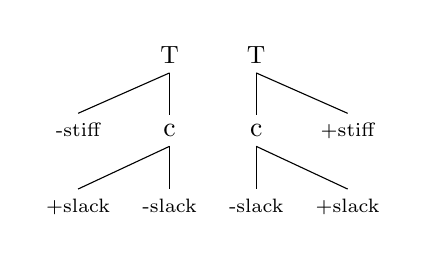
\begin{tikzpicture} [baseline = (z1.base)]
\matrix (m) [matrix of nodes, column sep = .5em, row sep = 1.5em]{
& \node(y1){\small T}; &  \node(y2){\small T}; \\
\node(z1){\scriptsize -stiff}; & \node(z2){c}; & \node(z3){c}; & \node(z4){\scriptsize +stiff}; \\
\node(t1){\scriptsize +slack}; & \node(t2){\scriptsize -slack}; &  \node(t3){\scriptsize -slack}; & \node(t4){\scriptsize +slack}; \\
};
\draw (z1.north) -- (y1.south);
\draw (z2) -- (y1.south);
\draw (z2.south) -- (t1.north);
\draw (z2.south) -- (t2);
\draw (y2) -- (z3);
\draw (y2.south) -- (z4.north);
\draw (z3) -- (t3);
\draw (z3.south) -- (t4.north);
\end{tikzpicture}
\hspace{.3cm}
$\rightarrow$
\hspace{.3cm}
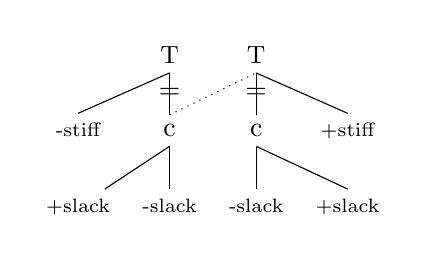
\begin{tikzpicture} [baseline = (z1.base)]
\matrix (m) [matrix of nodes, column sep = .5em, row sep = 1.5em]{
& \node(y1){\small T}; &  \node(y2){\small T}; \\
\node(z1){\scriptsize -stiff}; & \node(z2){c}; & \node(z3){c}; & \node(z4){\scriptsize +stiff}; \\
\node(t1){\scriptsize +slack}; & \node(t2){\scriptsize -slack}; &  \node(t3){\scriptsize -slack}; & \node(t4){\scriptsize +slack}; \\
};
\draw (z1.north) -- (y1.south);
\path (z2) edge node{=} (y1);
\draw (z2.south) -- (t1);
\draw (z2) -- (t2);
\path (z3) edge node{=} (y2);
\draw (y2.south) -- (z4.north);
\draw (z3) -- (t3.north);
\draw (z3.south) -- (t4.north);
\draw [dotted] (z2.north) -- (y2.south);
\end{tikzpicture}
\end{center}
We can represent this processes as a logical transduction from a Bao model input to a Bao model output. The input will be a disyllabic sequence /LM.HL/, that is, a low-registered rising contour syllable followed by a high-registered falling contour syllable. This model specification includes some changes in notation that will allow for a more direct comparison between the models in the qualifying paper itself: the register feature [$\pm$stiff] is designated [$\pm$u] for upper and lower registers, and the tonal feature [$\pm$slack] is designated [l] and [h] respectively by convention. Additionally, we impose a linear order over tier-internal elements via a binary successor function $succ$; this order is total such that the final element on a tier is its own successor. The input model for the Zhenhai case in Bao's tonal geometry $\mathcal{M}^{B}_{zh}$ is defined over the alphabet $\Sigma = \{\sigma, T, +u, -u, c, h, l\}$ below.
\begin{equation}
\begin{aligned}
\mathcal{M}^{B}_{zh}&\myeq\langle \mathcal{D},P_{\sigma},P_{T},P_{+u},P_{-u},P_{c},P_{h},P_{l},\alpha(x),\delta(x),succ(x)\rangle
\end{aligned}
\end{equation}
\begin{equation}
\begin{aligned}
\mathcal{D}&=\{1-12\} & P_{\sigma}&=\{1,2\} & P_{T}&=\{3,4\} \\
P_{-u}&=\{5\} & P_{+u}&=\{8\} & P_{c}&=\{6,7\} \\
P_{h}&=\{10,11\} & P_{l}&=\{9,12\} & \\
\delta(x)&=\begin{cases} 3 & x\in\{5,6\} \\ 4 & x\in\{7,8\} \\ 6 & x\in\{9,10\} \\ 7 & x\in\{11,12\}\end{cases} & \alpha(x)&=\begin{cases} 3 & x=1 \\ 4 & x=2\end{cases} & succ(x)&=\begin{cases} 2 & x\in\{1,2\} \\ 4 & x\in\{3,4\} \\ 8 & x\in\{5,8\} \\ 7 & x\in\{6,7\} \\ 10 & x=9 \\ 11 & x=10 \\ 12 & x\in\{11,12\}\end{cases}\\
\end{aligned}
\end{equation}
A graphical representation of this model is presented below. The successor function (`$\vartriangleleft$') is indicated using dotted lines. Note that no linear order is imposed on register and `c' nodes via this function, despite their shared sisterhood under a single `T' root node.
\begin{center}
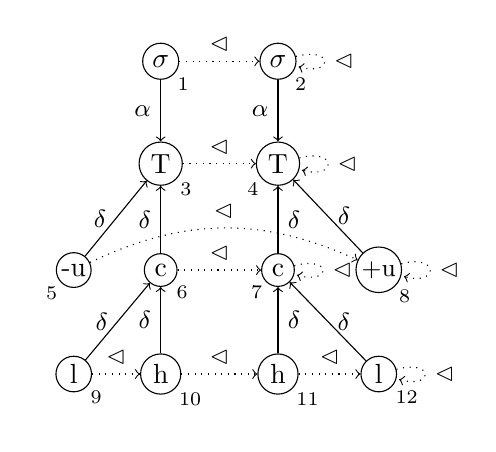
\begin{tikzpicture}[baseline = (x1.base)]
\matrix (m) [matrix of nodes, column sep = 1em, row sep = 1.5em]{
& \node[draw,circle, inner sep =2pt,label ={[label distance = -3pt] below right:\scriptsize$1$}](x1){$\sigma$};  &  \node[draw,circle, inner sep =2pt,label ={[label distance = -3pt] below right:\scriptsize$2$}](x2){$\sigma$}; \\
& \node[draw,circle, inner sep =2pt,label ={[label distance = -3pt] below right:\scriptsize$3$}](y1){T}; &   \node[draw,circle, inner sep =2pt,label ={[label distance = -3pt] below left:\scriptsize$4$}](y2){T}; \\
\node[draw,circle, inner sep =1pt,label ={[label distance = -3pt] below left:\scriptsize$5$}](z1){-u}; & \node[draw,circle, inner sep =2pt,label ={[label distance = -3pt] below right:\scriptsize$6$}](z2){c}; &   \node[draw,circle, inner sep =2pt,label ={[label distance = -3pt] below left:\scriptsize$7$}](z3){c}; & \node[draw,circle, inner sep =1pt,label ={[label distance = -3pt] below right:\scriptsize$8$}](z4){\se u}; \\
\node[draw,circle, inner sep =2pt,label ={[label distance = -3pt] below right:\scriptsize$9$}](t1){l}; & \node[draw,circle, inner sep =2pt,label ={[label distance = -3pt] below right :\scriptsize$10$}](t2){h}; &  \node[draw,circle, inner sep =2pt,label ={[label distance = -3pt] below right:\scriptsize$11$}](t3){h}; & \node[draw,circle, inner sep =2pt,label ={[label distance = -3pt] below right:\scriptsize$12$}](t4){l}; \\
};
\draw [->] (x1) -- (y1) node[left, pos=.5]{\small $\alpha$};
\draw [->] (x2) -- (y2) node[left, pos=.5]{\small $\alpha$};
\draw [->] (z1) -- (y1) node[left, pos=.5]{\small $\delta$};
\draw [->] (z2) -- (y1) node[left, pos=.5]{\small $\delta$};
\draw [->] (z3) -- (y2) node[right, pos=.5]{\small $\delta$};
\draw [->] (z4) -- (y2) node[right, pos=.5]{\small $\delta$};
\draw [->] (t1) -- (z2) node[left, pos=.5]{\small $\delta$};
\draw [->] (t2) -- (z2) node[left, pos=.5]{\small $\delta$};
\draw [->] (t3) -- (z3) node[right, pos=.5]{\small $\delta$};
\draw [->] (t4) -- (z3) node[right, pos=.5]{\small $\delta$};
\draw [->, dotted] (x1) -- (x2) node[above, pos=.5]{\small $\vartriangleleft$};
\draw [->, dotted] (y1) -- (y2) node[above, pos=.5]{\small $\vartriangleleft$};
\draw [->, dotted] (z2) -- (z3) node[above, pos=.5]{\small $\vartriangleleft$};
\path [->, dotted] (z1) edge[bend left=25] node[above, pos=.5]{\small $\vartriangleleft$} (z4);
\draw [->, dotted] (t1) -- (t2) node[above, pos=.5]{\small $\vartriangleleft$};
\draw [->, dotted] (t2) -- (t3) node[above, pos=.5]{\small $\vartriangleleft$};
\draw [->, dotted] (t3) -- (t4) node[above, pos=.5]{\small $\vartriangleleft$};
\path [->, dotted] (x2) edge[loop right] node{\small $\vartriangleleft$}(x2);
\path [->, dotted] (y2) edge[loop right] node{\small $\vartriangleleft$}(y2);
\path [->, dotted] (z4) edge[loop right] node{\small $\vartriangleleft$}(z4);
\path [->, dotted] (z3) edge[loop right] node{\small $\vartriangleleft$}(z3);
\path [->, dotted] (t4) edge[loop right] node{\small $\vartriangleleft$}(t4);
\end{tikzpicture}
\end{center}
To distinguish the `c'/terminal tonal nodes on the first and second syllables, we define two auxiliary relations which identify penults and ultima in a given string.
\begin{equation}
\begin{aligned}
last(x)&\myeq succ(x) = x \\
pnlt(x)&\myeq last(succ(x))\land \neg last(x) \\
\end{aligned}
\end{equation}
As before, the transduction defines the relations/functions of the output signature (a Bao model) in terms of the logical language of the input signature (a Bao model). No modification of TBU, root or register nodes obtains in the transduction; therefore the unary relations labeling these nodes are defined identical to the input. The `c' and terminal nodes from the first syllable only are generated in the output, so their unary relations are defined as: 
\begin{equation} \label{unary}
\begin{aligned}
P'_{c}(x)&\myeq P_{c}(x)\land pnlt(x) \\
P'_{h}(x)&\myeq P_{h}(x)\land pnlt(\delta(x)) \\ 
P'_{l}(x)&\myeq P_{l}(x)\land pnlt(\delta(x)) \\
\end{aligned}
\end{equation}
These definitions preserve the penultimate `c' node and the terminal nodes which are \emph{dominated by the penult} ($pnlt(\delta(x))$), that is, the c-terminal complex from the first syllable only. \par
Definition of binary functions follows a similar procedure. Association is preserved from the input, as is tier-internal linear order; we leave details of those definitions for the qualifying paper. Here, we focus on the definition of dominance ($\delta(x)\ap y$) which is crucial to modeling the shift process.
\begin{equation} \label{dominance}
\begin{aligned}
\delta'(x)\ap y&\myeq \big[\delta(x)\ap y\land P_{[-u]}(x)\land P_{T}(y)\big]\lor \\
&\quad\big[\delta(x)\ap y\land P_{[+u]}(x)\land P_{T}(y)\big]\lor \\
&\quad\big[P_{h}(x)\land P_{c}(y)\land pnlt(\delta(x)) \land pnlt(y)\big]\lor \\
&\quad\big[P_{l}(x)\land P_{c}(y)\land pnlt(\delta(x)) \land pnlt(y)\big]\lor \\
&\quad\big[P_{c}(x)\land P_{T}(y)\land pnlt(x) \land last(y)\big] \\
\end{aligned}
\end{equation}
Dominance is defined as five disjuncts. The first two preserve dominance relations between register and tonal root nodes from the input. Conjuncts three and four retain input dominance relations between terminal and `c' nodes from the penultimate (`first') syllable only, mirroring the definitions of the unary predicates $P'_{c}(x)$, $P'_{h}(x)$, and $P'_{l}(x)$. The final conjunct defines the rightward shift of contour; the penultimate `c' node is immediately dominated by the final `T' root.\par
The transduction is represented graphically as below. Successor relations are omitted. 
\begin{center}
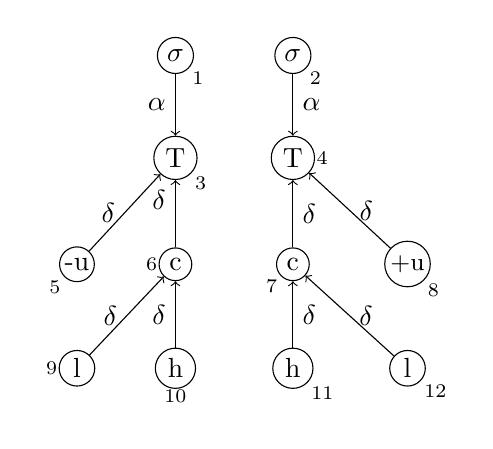
\begin{tikzpicture}[baseline = (y1.base)]
\matrix (m) [matrix of nodes, column sep = 1.5em, row sep = 1.5em]{
& \node[draw,circle, inner sep =2pt,label ={[label distance = -3pt] below right:\scriptsize$1$}](x1){$\sigma$};  &  \node[draw,circle, inner sep =2pt,label ={[label distance = -3pt] below right:\scriptsize$2$}](x2){$\sigma$};  \\
& \node[draw,circle, inner sep =2pt,label ={[label distance = -3pt] below right:\scriptsize$3$}](y1){T}; &   \node[draw,circle, inner sep =2pt,label ={[label distance = -3pt] right:\scriptsize$4$}](y2){T}; \\
\node[draw,circle, inner sep =1pt,label ={[label distance = -3pt] below left:\scriptsize$5$}](z1){-u}; & \node[draw,circle, inner sep =2pt,label ={[label distance = -3pt] left:\scriptsize$6$}](z2){c}; &   \node[draw,circle, inner sep =2pt,label ={[label distance = -3pt] below left:\scriptsize$7$}](z3){c}; & \node[draw,circle, inner sep =1pt,label ={[label distance = -3pt] below right:\scriptsize$8$}](z4){\se u}; \\
\node[draw,circle, inner sep =2pt,label ={[label distance = -3pt] left:\scriptsize$9$}](t1){l}; & \node[draw,circle, inner sep =2pt,label ={[label distance = -3pt] below :\scriptsize$10$}](t2){h}; &  \node[draw,circle, inner sep =2pt,label ={[label distance = -3pt] below right:\scriptsize$11$}](t3){h}; & \node[draw,circle, inner sep =2pt,label ={[label distance = -3pt] below right:\scriptsize$12$}](t4){l}; \\
};
\draw [->] (x1) -- (y1) node[left, pos=.5]{$\alpha$};
\draw [->](x2) -- (y2) node[right, pos=.5]{$\alpha$};
\draw [->](z1) -- (y1) node[left, pos=.5]{$\delta$};
\draw [->](z2) -- (y1) node[left, pos=.7]{$\delta$};
\draw [<-](z2) -- (t1) node[left, pos=.5]{$\delta$};
\draw [<-](z2) -- (t2) node[left, pos=.5]{$\delta$};
\draw [<-](y2) -- (z4) node[right, pos=.5]{$\delta$};
\draw [<-](y2) -- (z3) node[right, pos=.5]{$\delta$};
\draw [<-](z3) -- (t3) node[right, pos=.5]{$\delta$};
\draw [<-](z3) -- (t4) node[right, pos=.5]{$\delta$};
\end{tikzpicture}
\hspace{.5cm}
$\mapsto$
\hspace{.5cm}
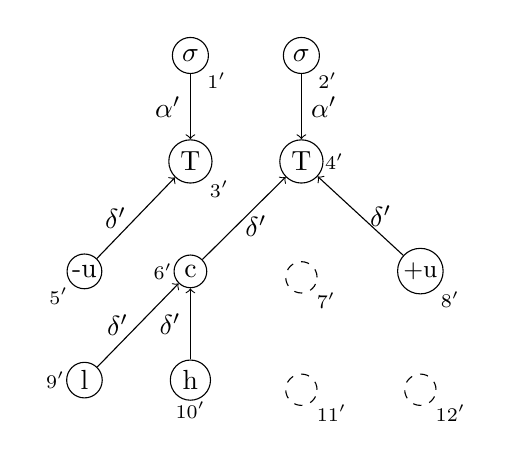
\begin{tikzpicture}[baseline = (y1.base)]
\matrix (m) [matrix of nodes, column sep = 1.5em, row sep = 1.5em]{
& \node[draw,circle, inner sep =2pt,label ={[label distance = -3pt] below right:\scriptsize$1'$}](x1){$\sigma$};  &  \node[draw,circle, inner sep =2pt,label ={[label distance = -3pt] below right:\scriptsize$2'$}](x2){$\sigma$};  \\
& \node[draw,circle, inner sep =2pt,label ={[label distance = -3pt] below right:\scriptsize$3'$}](y1){T}; &   \node[draw,circle, inner sep =2pt,label ={[label distance = -3pt] right:\scriptsize$4'$}](y2){T}; \\
\node[draw,circle, inner sep =1pt,label ={[label distance = -3pt] below left:\scriptsize$5'$}](z1){-u}; & \node[draw,circle, inner sep =2pt,label ={[label distance = -3pt] left:\scriptsize$6'$}](z2){c}; &   \node[draw,circle, dashed, inner sep =4pt,label ={[label distance = -3pt] below right:\scriptsize$7'$}](z3){\hspace{1em}}; & \node[draw,circle, inner sep =1pt,label ={[label distance = -3pt] below right:\scriptsize$8'$}](z4){\se u}; \\
\node[draw,circle, inner sep =2pt,label ={[label distance = -3pt] left:\scriptsize$9'$}](t1){l}; & \node[draw,circle, inner sep =2pt,label ={[label distance = -3pt] below :\scriptsize$10'$}](t2){h}; &  \node[draw,circle, dashed, inner sep =4pt,label ={[label distance = -3pt] below right:\scriptsize$11'$}](t3){\hspace{1em}}; & \node[draw,circle, dashed, inner sep =4pt,label ={[label distance = -3pt] below right:\scriptsize$12'$}](t4){\hspace{1em}}; \\
};
\draw [->] (x1) -- (y1) node[left, pos=.5]{$\alpha'$};
\draw [->](x2) -- (y2) node[right, pos=.5]{$\alpha'$};
\draw [->](z1) -- (y1) node[left, pos=.5]{$\delta'$};
\draw [->](z2) -- (y2) node[right, pos=.4]{$\delta'$};
\draw [<-](z2) -- (t1) node[left, pos=.5]{$\delta'$};
\draw [<-](z2) -- (t2) node[left, pos=.5]{$\delta'$};
\draw [<-](y2) -- (z4) node[right, pos=.5]{$\delta'$};
\end{tikzpicture}
\end{center}
Definitions of unary relations preserve the contour and terminal nodes from the first syllable, effectively `deleting' those from the second syllable. Additionally, immediate dominance holds relations constant from the input, with the exception of c-to-T dominance; penultimate `c' is dominated by final `T'. These modifications to the input structure are definable using Quantifier-Free First Order logic.
\subsection{Unifying Intertranslatability and Empirical Predictions}
So far, this section has outlined a methodological framework for comparing Bao and Yip tonal geometries, along the dimensions of their (potential) intertranslatability and empirical predictions. Both types of comparison are performed using logical transductions. We have already shown the advantages of such an approach; setting a threshold on complexity allows us to quantify notational equivalence of structure and formalizability of process in a principled way, that is, at some explicit level of logical complexity. Thus, intertranslatability by itself is not the evidence for notational equivalence, but rather intertranslatability \emph{at QF}. The same is true for processes. \par
We define two notationally equivalent models as those which are intertranslatable (same abstract properties, but differ only superficially) and share empirical coverage, and for which these properties are symmetrical between both representations. Another benefit of our methodological framework is that allows us to reason over these properties \emph{using the same formal language}. That is to say, this formalism unifies feature-geometric descriptions of representation and procedural descriptions of tonal processes (such as spread and delink). This is especially useful in light of the discussion about logical complexity; we can examine both properties in the same formal language and under the same threshold of logical complexity. The result is a principled and formally-rigorous comparison of the two tonal geometries.
\section{Remaining Work and Research Plan}
The Zhenhai transduction in Bao's representation from the previous section is QF-definable. The same has been asserted regarding the transductions between the models (\S5.2). These facts are of interest to the current research question and topic of the qualifying paper; the Zhenhai contour spreading pattern is said to be predicted by Bao's model but \emph{not} Yip's. If, however, logical transductions between model signatures are definable using a relatively weak logic (QF), and if the process itself as a transduction can be represented in logically simple terms (also QF), is it still possible to say that it cannot be formalized in Yip's model? Given the translatability of the models, what would it mean for one process to be formalizable in one representation and not the other? We explore this issue further in the qualifying paper, with the goal of demonstrating that, if the models are intertranslatable, there is no process that can be represented in one geometry and not the other. Here, we discuss the work that remains to achieve that goal in the qualifying paper, and how to go about it.\par
First, we must provide QF-definable transductions between the models (this has been done already) to demonstrate their intertranslatability. This alone, however, does not guarantee that the models make the same empirical predictions (for processes at the QF threshold). Consider the schema below:
\begin{center}
\begin{tabular}{ccccc}
& & {\small$\tau^{B}_{zh}$} \\
& $\mathcal{M}^{B}_{I}$ & {\Large$\mapsto$} & $\mathcal{M}^{B}_{O}$ \\
\hspace{1em} \\
{\small$\Gamma^{by}$} & {\Large$\downmapsto$} & & {\Large$\downmapsto$} & {\small$\Gamma^{by}$} \\ 
\hspace{1em} \\
& $\mathcal{M}^{Y}_{I}$ & {\Large$\mapsto$} & $\mathcal{M}^{Y}_{O}$ \\
& & {\small\underline{$\tau^{Y}_{zh}$(QF?)}} \\
\end{tabular}
\end{center}
Using Zhenhai contour shift as an example, we can posit a QF-definable transduction $\tau^{B}_{zh}$ which, when given a Bao input model $\mathcal{M}^{B}_{I}$, will yield a corresponding output model $\mathcal{M}^{B}_{zh}$ in Bao's representation. Both the input and output structures can be translated into Yip-geometry analogs \emph{separately} via the QF-definable transduction $\Gamma^{by}$. This yields input $\mathcal{M}^{Y}_{I}$ and output $\mathcal{M}^{Y}_{O}$ models in Yip's representation. Given these facts, does it follow that there exists some QF-definable Zhenhai contour shift transduction $\tau^{Y}_{zh}$ that operates directly over Yip's representation? Not yet. To do so, we must prove that QF is closed under composition. While \citet{Courcelle1994} has proven this for logics of higher complexity (FO and MSO), no explicit proof has been sketched for QF. We will offer such a proof in the qualifying paper, and in doing so, will show that any QF-definable process in Bao's model can be represented in Yip's model and vice versa. In other words, the two models make the same empirical predictions at the QF threshold. \par
In the interest of thoroughness, we also define QF transductions for other tonal processes, crucially those which are argued to be formalizable in both representations. Such processes include spread/shift patterns that target register, whole contour tones, and terminal nodes; dissimilation and substitution; and neutralization. This offers further support for the claim that the models make the same empirical predictions. It also highlights what the structural analogs are in each respective representation given specific processes.
\section{Conclusion}
This qualifying paper has motivated a rigorous analysis of the notational equivalence of tonal geometries offered in Yip (1989) and Bao (1990), models which have been argued to be distinct representations which make different empirical predictions. We addressed the question of notational equivalence first by defining the notion explicitly: grammatical models are said to be equivalent when differences in their representation of abstract features is superficial, and when they make the same empirical predictions. Furthermore, equivalence must be symmetrical. \par
We further established a protocol for proving the equivalency of the models using the formalism of model theory, and outlined the advantages of this approach. Specifically, we use QF-definable logical transductions to translate between the models, as well as represent attested tonal processes which are claimed to be formalizable in one tonal geometry model but not the other. The benefit of this approach is three-fold. First, it quantifies `superficial' differences as those which permit translation using a low complexity threshold. Additionally, it constrains (also using QF) the possible space of `empirical predictions'--especially with respect to processes which are not fully understood--to facilitate a direct and principled comparison of the models' capacity to represent certain processes. Finally, it unites the notions of intertranslatability and empirical predictions by reasoning over them in the same formal language. Quantifier-Free logic is chosen as the logical threshold for this analysis as it is well-understood, restrictive, and has analogs elsewhere in phonology (see \S5.2).\par
Ideally, this qualifying paper will serve as a proof of concept to be expanded in future analyses. This may include expanding the empirical scope to other attested tonal processes (outside of Chinese tone sandhi) as well as other competing models of tonal representation which have been claimed to be distinct but may very well be notationally-equivalent.
\bibliographystyle{apalike}
\bibliography{references}
\end{document}